\documentclass[10pt,letterpaper]{article}
\usepackage[top=0.85in,left=2.0in,footskip=0.75in]{geometry}
\usepackage{amsmath,amssymb}
\usepackage{changepage}
\usepackage[utf8]{inputenc}
\usepackage{textcomp,marvosym}
\usepackage{cite}
\usepackage{nameref}
\usepackage[pdftex,
            pdfauthor={Peter Reintjes},
            pdftitle={Fitness Landscape Visualization},
            pdfsubject={MatPlotLib Visualization},
            pdfkeywords={Python Matplotlib},
            pdfproducer={Latex with hyperref},
            pdfcreator={pdflatex}]{hyperref}

\hypersetup{
    colorlinks=true,
    linkcolor=blue,
    filecolor=magenta,      
    urlcolor=cyan,
}
\usepackage[right]{lineno}
\usepackage{microtype}
\DisableLigatures[f]{encoding = *, family = * }
\usepackage[table]{xcolor}
\usepackage{array}
\usepackage{listings}
\newcolumntype{+}{!{\vrule width 2pt}}
\newlength\savedwidth
\newcommand\thickcline[1]{%
  \noalign{\global\savedwidth\arrayrulewidth\global\arrayrulewidth 2pt}%
  \cline{#1}%
  \noalign{\vskip\arrayrulewidth}%
  \noalign{\global\arrayrulewidth\savedwidth}%
}

% \thickhline command for thick horizontal lines that span the table
\newcommand\thickhline{\noalign{\global\savedwidth\arrayrulewidth\global\arrayrulewidth 2pt}%
\hline
\noalign{\global\arrayrulewidth\savedwidth}}

\usepackage{enumitem}
\setlist{nosep}
\raggedright
\setlength{\parindent}{0.5cm}
\textwidth 5.25in 
\textheight 8.75in

\usepackage[aboveskip=1pt,labelfont=bf,labelsep=period,justification=raggedright,singlelinecheck=off]{caption}
\renewcommand{\figurename}{Fig}

% Remove brackets from numbering in List of References
\makeatletter
\renewcommand{\@biblabel}[1]{\quad#1.}
\makeatother

% Leave date blank
\date{}
% Header and Footer with logo
\usepackage{lastpage,fancyhdr,graphicx,wrapfig}
\usepackage{epstopdf}
\pagestyle{myheadings}
\pagestyle{fancy}
\fancyhf{}
\setlength{\headheight}{27.023pt}
%\lhead{\includegraphics[width=2.0in]{PLOS-submission.eps}}
%\rfoot{\thepage/\pageref{lastpage}}
\renewcommand{\footrule}{\hrule height 2pt \vspace{2mm}}
\fancyheadoffset[L]{2.25in}
\fancyfootoffset[L]{2.25in}
% customize
\lfoot{\sf Innatrix Internal Document}

\begin{document}

\title{Fitness Landscape Animation Software}
\author{Peter Reintjes}
\date{\today}
\maketitle

\vspace*{0.2in}
\begin{flushleft}
\includegraphics[scale=0.5]{{fitness}.png}
\end{flushleft}

{\it Continuous Directed Evolution can be visualized by showing mutations as entities crawling across a fitness landscape until they come to a particular height on a fitness peak.  The two-dimensional surface is an imperfect representation of sequence space, which could be thought of as NxM dimensional space for the M possible substitutions for each of the N amino acids making up the protein sequence.  For a 1000 amino acid protein, this surface would have on the order of $21^{1000}$ points and would probably be quite spikey, as sequences close to each other in terms of mutations would not in general have similar 'fitness'.  For this reason, we portray a fictional two-dimensional surface in which 'nearby' variants have similar 'fitness'.  On the other hand, for directed evolution, because the fitness itself is a single dimension (protein-protein affinity, or enzymatic activity) it is well represented by a height.  Thus the term fitness-peak is commonly used to represent a maxima in this space.  We use the Python matplotlib library\cite{matplotlib} program to create a series of static images, representing a particular population of mutations at one point in time and then assembled these into an animated GIF image to visualize the process of evolution.  This method was inspired by the animations created by Randy Olsen and Bjorn Ostman which can be found near the bottom of the {\bf Wikipedia} entry on Fitness Landscape\cite{fitness}. The present program was created because Olsen and Ostman did not describe how they produced their animation.}

\section*{Introduction}

The {\bf landscape.py} program is a Python program which generates a series of images representing snapshots of protein evolution in an imagined three-dimensional fitness landscape.

\section*{Reasons for using the Python MatPlotLib module}

\begin{enumerate}[itemsep=1pt, topsep=2pt, partopsep=0pt]
\item Python/Matplotlib is free
\item Python/Matplotlib is portable between Windows and Linux systems
\item Skilled Python Programmers are becoming more numerous
\item Python was already in use for the EvoStat project
\item The MatLab/Octave alternative required an additional learning curve and those languages did not seem to suit other general purpose needs of the overall project.
\end{enumerate}
Although Octave, as an open-source alternative to MatLab is free and portable between systems, I decided to go with Python after initially prototyping in Octave.

\subsection*{Viewing the Animations}
Four versions of the animation are currently available from the EvoStat (Tor) web interface.  The main page now has four additional links which link to the labeled and unlabeled animation with white or black backgrounds. While viewing an animation, clicking on it will toggle between the labeled and unlabeled versions.
\subsection*{Downloading}
The source code and this documentation are on GitHub at {\bf https://github.com/eatoin5hrdlu/landscape.git}.
\subsection*{Requirements}
\subsubsection*{Python Modules}
The list of Python dependencies is large and setting up the Python environment to have compatible versions of all required libraries was a substantial was a non-trivial aspect of this task.
\begin{lstlisting}
from __future__ import print_function
import numpy as np
import mpl_toolkits.mplot3d as a3
import pylab as pl
import scipy as sp
import matplotlib.pyplot as plt
import matplotlib.patches as mpatches
import matplotlib.colors as colors
import matplotlib
import random, glob, os, subprocess, sys
from shutil import copyfile
from mpl_toolkits.mplot3d import Axes3D
from matplotlib.colors import LightSource
\end{lstlisting}
\subsubsection*{ImageMagick}
As soon as the program has produced ten static frames, it will call the ImageMagic\cite{imagemagick} {\tt convert} command to produce an animated GIF. It will call this program whenever ten additional frames have been generated. The still frames can be previewed in the temp directory: {\bf /tmp/gifmovie/000NN.png} and the latest animation in the file {\bf /tmp/gifmovie/evolution.gif}.
\begin{lstlisting}
{convert 0*.png -delay 12 -gravity Center -crop 500x280+20-20! evolution.gif
\end{lstlisting}
Which collects all of the properly cropped {\bf .png} files (in the /tmp/gifmovie directory) into an animated GIF with 12ms per frame.  This external command is called via the Python subprocess module, but could presumably be done using the PythonMagick bindings.  As this would also provide access to the other image enhancement features of ImageMagick this may be worth serious consideration.

\subsection*{Markers}
I chose the 'o' (circle), 'D' (diamond), and 's' (square) markers to represent the mutants, global maximum fitness peak, and landscape origin. But other markers could be chosen. There is an interesting outstanding problem with z-ordering the markers when drawn on top of a 3D surface.

\begin{wrapfigure}{L}{0.25\textwidth}
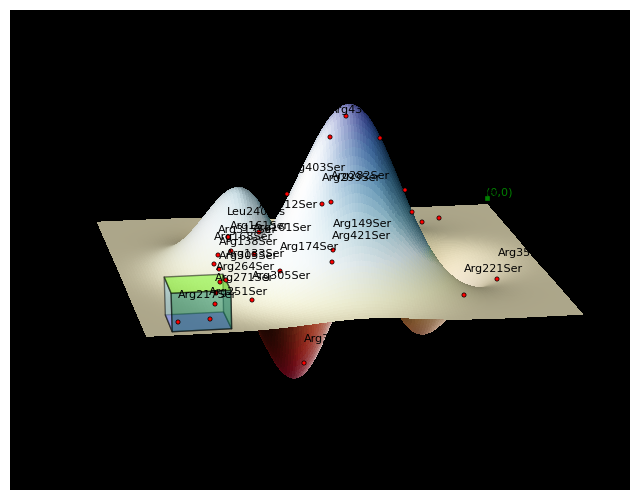
\includegraphics[width=0.23\textwidth,scale=0.2]{fitness.png}
\caption{\label{fig:reticules}A Single Snapshot}
\end{wrapfigure}

\subsection*{Miscellaneous Decorations}
Marshall asked for a box representing ``the machine'', or more generally, our process for producing mutants, so I've explored the creation of an arbitrary decorative objects.  Think of things which are not data-point in the graph, but we want to be in the picture anyway.   A collection of colored polygons can be created and added to the plot, although it takes a bit of tweaking with the {\bf zorder} and {\bf zsort} options to make sure it is drawn in front of, or behind, other objects as needed.  I spent a bit of time figuring out how to create the flashing multi-colored box which sits in the corner of the 3D fitness landscape graph and serves as the genesis point for new mutations.

\subsection*{Labeled Animations}
For every animation, I've created a labeled and unlabeled versions.  Along with little red mites representing mutations that run around with a combination of Brownian motion and hill-climbing, the program generates an optional label representing a mutation: AminoAcid-Position-AminoAcid, (e.g. Ser123Arg).   More than one mutation will make for cluttered label, so whether we end up using this for real (rather than just demo) mutations is a question.

\subsection*{Next Steps}
\begin{enumerate}[itemsep=1pt, topsep=2pt, partopsep=0pt]
\item 
Marshall suggested that the little box would generate mutants that would be able to climb a certain distance up the global peak before stalling out, and that a later mutation would come out of the box and climb higher. A more realistic representation would be for the mutant that had climbed part way up the hill would split into a copy and a mutant, and that the mutant would either climb higher or slip lower on the peak. The one slipping lower would wink out some time later, while the one climbing would stall at a higher altitude before splitting again.  It sounds complicated, but isn't necessarily harder to produce than the thing Marshall asked for, but seems to me to have an additional basis in reality. E.g., better mutants are not being generated at a location down away from the hillside of the fitness peak, but in fact on the slope.
\item I'm hoping to turn this project over to Dawn Trembath.
\item Add command-line options to avoid frequent program edits when generating different visualizations.
\item Consider cost/benefits of using PythonMagick bindings instead of external call to convert program (to generate GIFs)
\item Add option to produce longer movies in formats other than GIF (mp4, mpeg, etc.)
\end{enumerate}

\bibliographystyle{unsrt}
\bibliography{landscape}{}

\pagebreak

\section{Appendix: landscape.py source code}
\newcommand*{\SrcPath}{..}
\lstinputlisting[language=Python]{\SrcPath/mlandscape.py}
\end{document}
